\subsection{Approximating the distance function}
\label{sec:dist smoothing}
To create a smooth approximation to $\robf$, we use smooth approximations to each of its non-differentiable components: the set-distance, min, and max functions.

\begin{figure}[t!]
	\centering
	\begin{subfigure}[t]{0.25\textwidth}
		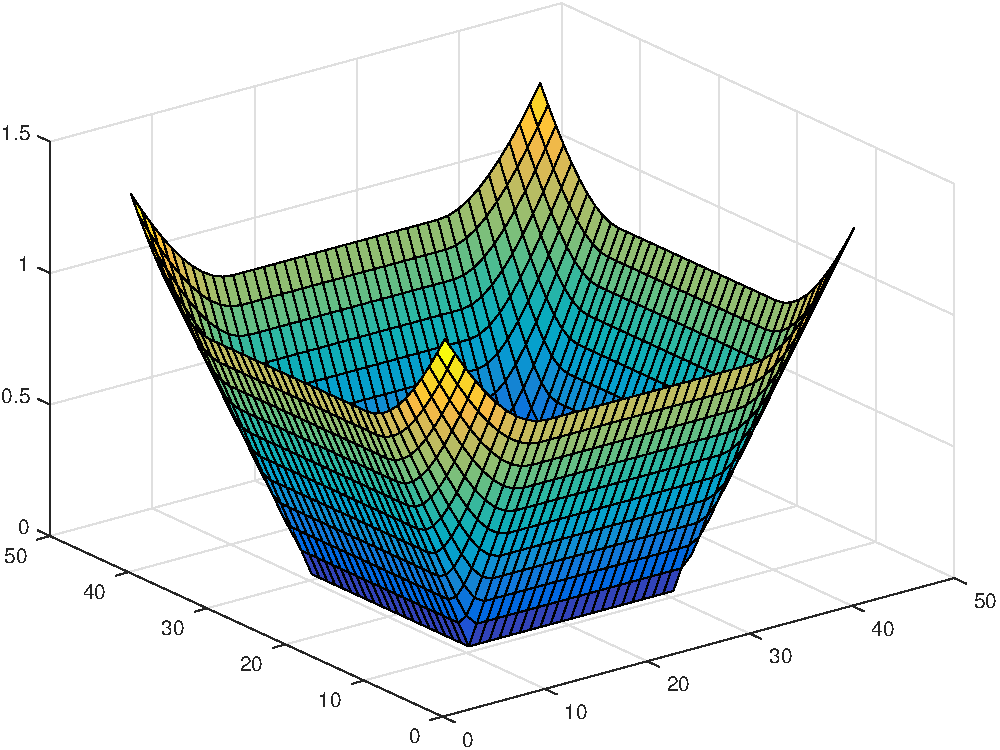
\includegraphics[height=1.2in]{figures/smoothDist2d}
		\caption{Smoothed function}
	\end{subfigure}%
	~
	\begin{subfigure}[t]{0.25\textwidth}
		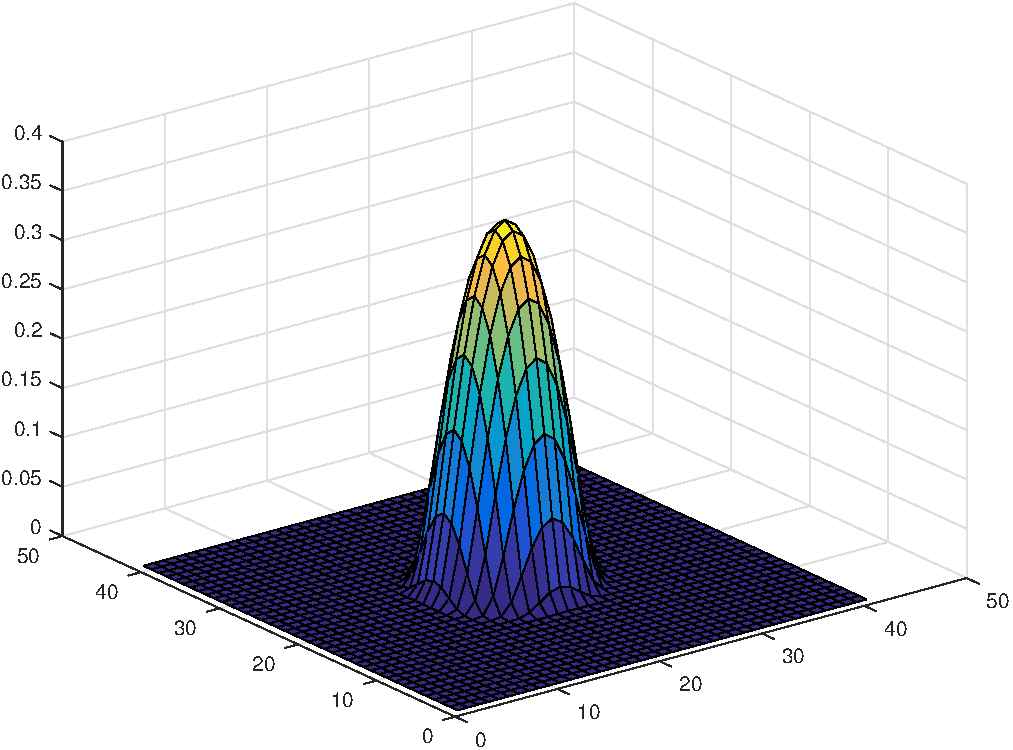
\includegraphics[height=1.2in]{figures/kernelG}
		\caption{Function $g$}
	\end{subfigure}
	\caption{{\small Smoothed 2-d distance function to a square in the x-y plane, and the function $g$ used to smoothen it.}}
	\vspace{-20pt}
	\label{fig:smooth2d}
\end{figure}

Recall that for a set $U \subset \Re^n$, $\dist(x,U) = \inf_{a \in \cl{U}} |x-a|_2$, where $|\cdot|_2$ is the Euclidian norm.
This function is globally Lipschitz with Lipschitz constant 1 and therefore differentiable almost everywhere (Rademacher's theorem), and has a second derivative almost everywhere if $U$ is convex (Alexandrov's theorem) \cite{MakelaN92book}.

It is well-known that if we convolve an a.e.-differentiable function with a smooth kernel, the output function no longer has those singularities.
We give an example of such a construction, which lays the groundwork for explaining the more general wavelet-based smoothing we use in the experiments.
$C^\infty(\Re^n)$ is the class of functions that are infinitely differentiable in $\Re^n$.
\begin{theorem}
	\label{thm:ge smoothing}
	Consider the globally Lipschitz function $f:\Re^n \rightarrow \Re$ with Lipschitz constant $L_f$.
	Let $g: \Re^n \rightarrow \Re_+$ be a non-negative $C^\infty(\Re^n)$ function that integrates to 1 and is supported on the unit ball:
	$\int_{\Re^n}g(x)dx = 1$, $g(x) = 0$ if $x \notin B(0,1)$.
	Define $g_\varepsilon = \varepsilon^{-n}g(x/\varepsilon)$ and
	\[f_\varepsilon(x) = f *g_\varepsilon(x) = \int_{\Re^n}f(y)g_\varepsilon(x-y)dy\]
	Then $\fe$ is infinitely differentiable, its Lipschitz constant $L_{\fe} \leq L_f$ and $\|f-\fe\|_\infty \leq L_f \varepsilon$.
\end{theorem}
\begin{proof}
	Clearly, $\fe$ is $C^\infty$: $g_\varepsilon \in C^\infty$ and the integrand in the above convolution is differentiable w.r.t. $x$, so it holds that $\fe'(x) = \int{f(y)\partial g_\varepsilon(x-y)/\partial x dy}$.
	
	Convolution is commutative so $f_\varepsilon(x) = \int_{\Re^n}f(x-y)g_\varepsilon(y)dy$.
	Let $x' \in \Re^n$, then 
	\begin{eqnarray*}
	|\fe(x)-\fe(x')| &=& |\int_{\Re^n} f(x-y)g_\varepsilon(y) - f(x'-y)g_\varepsilon(y) dy|
	\\
	&\leq & \int_{\Re^n} g_\varepsilon(y)|f(x-y) - f(x'-y)| dy
	\\
	& = & L_f|x-x'| \int_{\Re^n} \varepsilon^{-n} g(y/\varepsilon) dy
	\\
	&= &L_f|x-x'| \int_{\Re^n} \varepsilon^{-n} g(y') \varepsilon^ndy'
	\\
	&=& L_f|x-x'| \implies L_f \leq L_{\fe}
	\end{eqnarray*}
	
	Finally, 
	\begin{eqnarray*}
	|\fe(x)-f(x)| &=& \left|\int_{\Re^n}f(x-y)g_\varepsilon(y)dy - \int_{\Re^n}f(x)g(y)dy\right|
	\\
	&=& \left|\int_{\Re^n}f(x-\varepsilon y)g(y)dy - \int_{\Re^n}f(x)g(y)dy\right|
	\\
	&\leq& \int_{B(0,1)}|f(x- \varepsilon y) - f(x)|g(y)dy	
	\\
	&\leq & \int_{B(0,1)}L_f | \varepsilon y| g(y)dy \leq L_f \varepsilon
	\end{eqnarray*}
	In particular, $\|f-\fe\|_\infty \rightarrow 0$ as $\varepsilon \rightarrow 0$.
\end{proof}
Fig.~\ref{fig:smooth2d} shows the distance function $\dist(\cdot,U)$ where $U$ is a square in the plane, smoothed by convolving with kernel $g_{\varepsilon}$ obtained from the shown function. 
We used $\varepsilon = 0.001$, and the actual approximation error $\|f-\fe\|_\infty$ is less than 1e-15.
Parameter $\varepsilon$ controls how peaked or flat $g_\varepsilon$ is: a large $\varepsilon$ gives a peaked kernel which yields better local approximation, but the max error decreases towards 0 slower.

%\todo[inline]{because lip cnt is bounded by that of f, this says that it's a conservative apx? if d is -ve and decreasing, $d_\varepsilon$ decreases less and if d is +ve and increasing, $d_e$ increases less.}

\subsection{Wavelet approximations}
\label{sec:waveletApx}

Wavelets can be viewed as a generalization of the kernel $g_\varepsilon$ of the previous section to a whole family of kernels, obtained by translations and dilations of one function called the `mother wavelet' $\psi$: $\psi_{k,j}(x) = \sqrt{2^{-j}}\psi(2^{-j}(x-k))$  \cite{MallatBook}.
They are used extensively in signal processing, as they have very good approximation properties, including fast convergence and multi-scale analysis.
See \cite{MallatBook}.
In the experiments in the rest of this paper, we used the Meyer wavelets. 
Specifically
\todo[inline]{Yash, meyer}
 
